\documentclass[fleqn, a4paper, 12pt]{article}
\usepackage[utf8]{inputenc}
\usepackage[T1]{fontenc}
\usepackage{lmodern}
\usepackage[left=0.5in, right=0.5in, top=0.5in, bottom=0.5in]{geometry}
\usepackage{mathexam}
\usepackage{amsmath}
\usepackage{graphicx}

\let\ds\displaystyle

\newcommand{\me}{\mathrm{e}}



\ExamClass{Logical computational thinking}
\ExamName{I partial example}
\ExamHead{28 September 2015}

\begin{document}
\ExamNameLine
\ExamInstrBox{Read carefully the problem, then identify the important
  parts, make a \textbf{model}, and a \textbf{flow chart}. Remember to
describe all the passages that brings you to give a certain answer (why
a certain value is an input, where you found information on the
data type, why you made a certain choice, etc\dots).}
\paragraph{Work:}
You have been contacted by the \emph{WHO}, they need to build a
software for calculating whether they are able to develop
an effective 
vaccine for a flu type in a certain period of time or not.

A simple mathematical model for the spreading of an infection in a
population is given by the equation:
\begin{equation}\label{eq:model}
  p(t) = \frac{100}{1+\frac{100-p_0}{p_0}\me^{-\lambda t}}
\end{equation}
where $p(t)$ is the percentage of the population infected
at a time $t$, expressed in days from now. $p_0$ is the percentage of the infected
population at time $t=0$ (now), and $\lambda$ is the virulence rate of
the virus in a certain 
population. The value of $\lambda$ can be between $0$ and $1$.
\begin{figure}[h]
  \begin{center}
    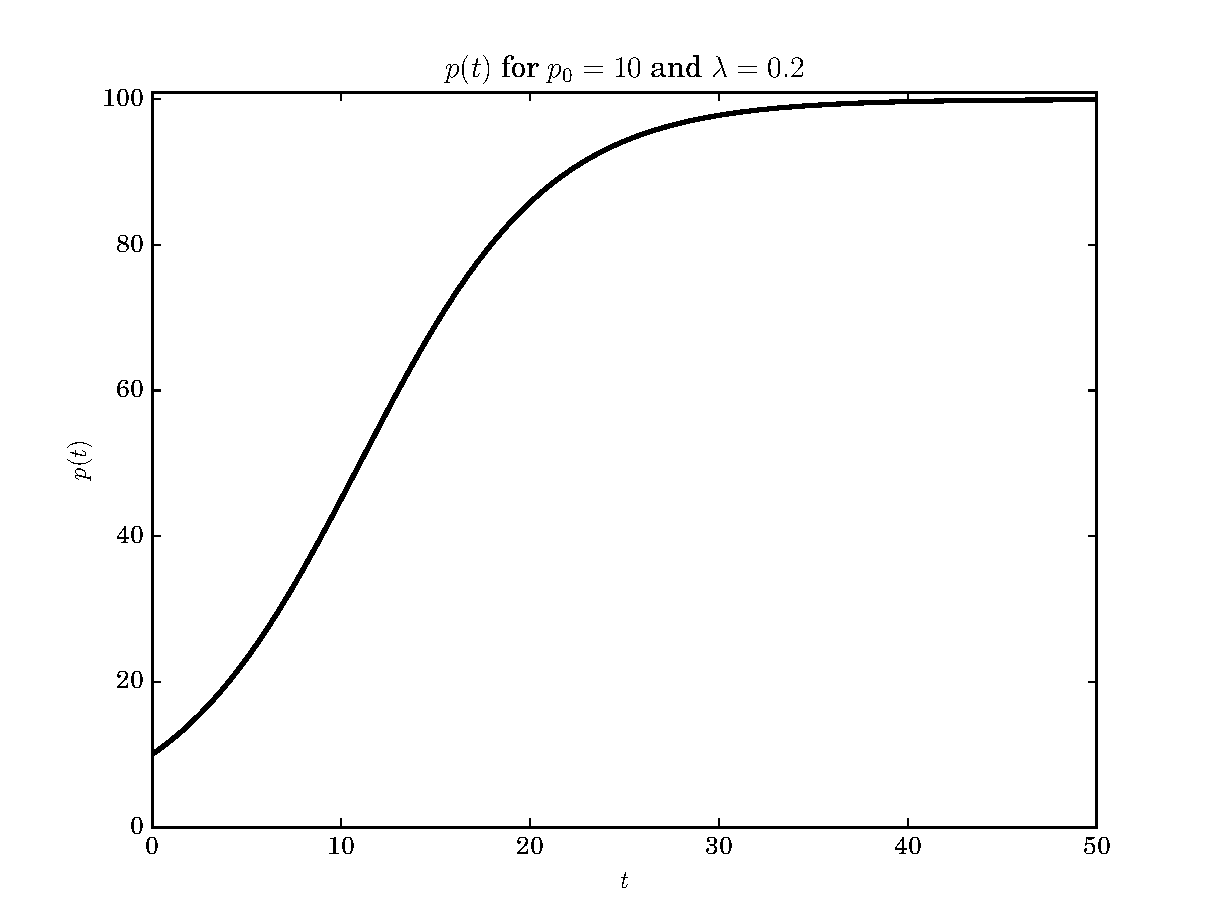
\includegraphics[width=.45\textwidth]{img/logistic.pdf}
    \caption{Example of equation (\ref{eq:model})}
    \label{fig:model}
  \end{center}
\end{figure}

When the \emph{WHO} discover a new ongoing flu infection they follow the steps:
\begin{enumerate}
\item study the pathogen;
\item study the population;
\item use the results of the previous studies to calculate a specific
  $\lambda$ rate for the infection;
\item calculate the percentage of the population infected at current time;
\item calculate the time to develop enough doses of vaccine for half
  the population, in days.
\end{enumerate}
At this point they need to use your program to determine if they
can develop the vaccine in time for half of the population, or if the
infection is faster than the time needed (more than half of the
population will be already infected when the vaccine will be ready).

\paragraph{Tip:}
You can use the equation~(\ref{eq:model}) to calculate if in a
certain time the infected population is less or more than the 50\%.
The output can be a \emph{``Yes''} if the \emph{WHO} can
develop the vaccines in time or a \emph{``No''} otherwise. 
\end{document}

